\chapter{Proposta de solução}

Neste capítulo serão apresentados os componentes e procedimentos utilizados na elaboração da proposta de solução, denominada de ``BURI''. Conforme as
etapas definidas na metodologia, ocorre inicialmente a discussão sobre a fase de pesquisa na Seção \ref{fase1}, seguida pela especificação 
das funcionalidades e comportamento do sistema BURI, contextualizados na Seção \ref{fase2}. O particionamento e execução de atividades nas áreas de 
\textit{hardware} e \textit{software} são explicados nas Seções \ref{fase3} e \ref{fase4}, respectivamente. Na Seção \ref{fase5},  o aplicativo Android e o 
dispositivo físico são avaliados por um grupo selecionado de alunos, a fim de garantir a usabilidade do sistema proposto e, posteriormente, são produzidas a documentação 
do projeto e guia de instalação na Seção \ref{fase6}. 

\section{Pesquisa}\label{fase1}

A primeira fase consiste na compreensão do problema. O objetivo é encontrar trabalhos semelhantes sobre o uso de IoT no monitoramento da qualidade do ar, assim 
como as consequências fisiológicas de inalação prolongada de monóxido de carbono, e identificar, através de um questionário aplicado aos alunos, as preocupações relacionadas 
à qualidade do ar no ambiente doméstico.

Em primeiro lugar, realizou-se uma revisão da literatura para identificar pesquisas no âmbito de tecnologias IoT e monitoramento do ar com foco 
em prevenção de acidentes, porém foram selecionados cinco trabalhos acadêmicos para o desenvolvimento deste projeto e comparação de funcionalidades. Em destaque, o 
trabalho de Sá considerou a detecção em tempo real do Gás Liquefeito de Petróleo (GLP) na residência \cite{uea-iot-deteccao-incendio}, atuando na prevenção de incêndio por vazamento de gás e servindo como referência para o desenvolvimento 
do \textit{hardware} do BURI. Por outro lado, o trabalho ``Intelligent based novel embedded system based IoT enabled
air pollution monitoring system'' \cite{tbRelacionado4NovelEmbeddedSystem} abordou uma arquitetura de comunicação em rede e processo de calibração de sensores
fundamental para o desenvolvimento do \textit{software} deste projeto de conclusão de curso.

Além disso, o estudo da intoxicação por monóxido de carbono visa investigar as consequências para a saúde humana. Portanto, a explicação científica sobre o tema é do 
artigo ``Carbon monoxide poisoning: a review for clinicians'' \cite{carbon-monoxide-poisoning-varon}, pois o conteúdo inclui 
explicação técnica e didática do processo de envenenamento, consequências no sistema neurológico e cardiovascular, fontes de contaminação e métodos de tratamento utilizados na medicina.

Por fim, um questionário foi aplicado aos alunos da Escola Superior de Tecnologia da Universidade do Estado do Amazonas (EST/UEA) para coletar informações sobre suas preocupações relacionadas à qualidade do ar no ambiente doméstico.
A pesquisa buscou identificar as configurações do ambiente residencial desses alunos e avaliar seu nível de conscientização sobre os riscos associados a poluentes no ar. Ao todo, 
58 estudantes das áreas de Engenharia responderam a este primeiro questionário.

Os resultados obtidos com as respostas trouxeram dados valiosos para a construção do protótipo. Em particular, algumas questões revelaram tendências e 
preocupações específicas, que serão analisadas a seguir. Segundo a pesquisa, 75,9\% dos estudantes utilizam um \textit{smartphone} com 
Sistema Operacional Android, pois a tecnologia representa uma importante fonte de acesso à informação e inclusão digital no Brasil \cite{impacto-android-brasil}. Outro aspecto analisado foi 
a percepção dos alunos em relação à qualidade do ar em suas residências e arredores. Nas respostas discursivas, foram frequentes os relatos sobre a presença de fumaça em dias específicos, 
atribuída às queimadas recorrentes na região de Manaus. Como relatou um dos alunos: ``a fumaça se tornou um problema pra resolver isso decidimos comprar um umidificador de ar''. 

Evidência dos relatos, a Universidade do Estado do Amazonas (UEA) suspende atividades presenciais nos dias 19 e 20 de setembro na capital e interior por causa 
da alta quantidade de poluentes, pois os índices ultrapassaram a marca de 125 $\mu m/m^{3}$ e um ar de boa qualidade permite a concentração de partículas em  até 25 $\mu m/m^{3}$ \cite{uea-queima-fecha}. 

\begin{figure}[ht]
    \centering
    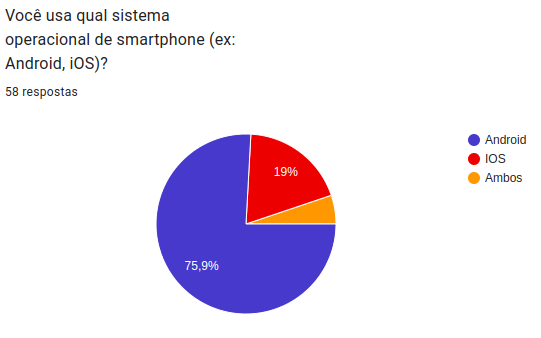
\includegraphics[width=.67\textwidth]{img/graf1-SO-smartphone.png}
    \caption{Sistemas Operacionais dos \textit{smartphones} dos alunos da EST. Fonte:Autor}\label{figSOsmartphone}
\end{figure}

A seguir, a figura \ref{figWifiAlunos} ilustra a porcentagem de estudantes com rede Wi-Fi em suas residências. Após essa análise, observou-se que 
a grande maioria possui acesso à rede Wi-Fi. Esse fator é especialmente relevante para a viabilidade do projeto, uma vez que a conectividade 
constante permitirá o funcionamento do sistema \textit{online}.

\begin{figure}[ht]
    \centering
    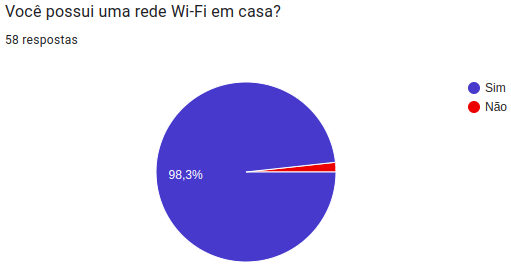
\includegraphics[width=.67\textwidth]{img/graf1-wifi.png}
    \caption{Uso de Wi-Fi dos alunos da EST. Fonte:Autor}\label{figWifiAlunos}
\end{figure}

\section{Especificação}\label{fase2}

A especificação é a etapa onde são definidas as funcionalidades do sistema embarcado e a modelagem da arquitetura e comunicação entre 
seus componentes. A partir das respostas ao questionário aplicado aos alunos, foram identificadas as principais funcionalidades esperadas 
para o sistema BURI, pois o desenvolvimento das especificações do sistema deve garantir que o protótipo final atenda às demandas reais do
público alvo. A funcionalidade de monitoramento em tempo real recebeu o maior número de votos entre os participantes, porém opções como alerta de risco, fácil instalação e 
manutenção mínima foram requisitos também muito solicitados no questionário. A justificativa para a preocupação com uso do equipamento é que apenas 37,9\% dos alunos já fizeram uso de 
algum dispositivo de automação residencial. Portanto, a solução da proposta deve focar em configurações simples para usuários sem experiência.
%Em segundo, existe a fase de especificação. Ocorre o levantamento de funcionalidades do sistema, com aplicação de questionário 
%e entrevistas para a compreensão do domínio de problema. Por outro lado, é realizada também a modelagem do circuito 
%eletrônico, arquitetura do \textit{software} de dados/alerta, fluxo de navegação do aplicativo móvel e, por fim, o 
%planejamento da comunicação entre o aplicativo e o dispositivo microcontrolador.
\begin{figure}[ht]
    \centering
    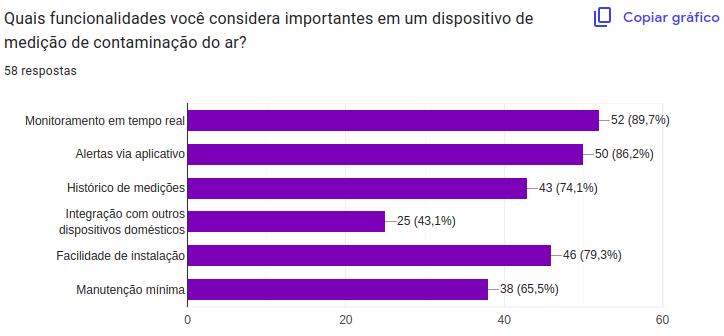
\includegraphics[width=.77\textwidth]{img/graf1-funcionalidades.png}
    \caption{Funcionalidades desejadas do sistema embarcado. Fonte:Autor}\label{figFuncionalidades}
\end{figure}

\section{Particionamento (Hw/Sw)}\label{fase3}

\section{Execução de Atividades}\label{fase4}

\section{Testes de aceitação}\label{fase5}

\section{Manutenção e atualização}\label{fase6}